% !TeX root = ../main.tex

\chapter{绪论}\label{chap:intro}

本章主要介绍本课题的研究背景与意义、研究现状以及本文的主要研究内容,最后将对本文的组织结构进行阐述。

\section{研究背景与意义}

\subsection{人工智能}

人工智能是指通过电子信息技术呈现出人类智能的技术,作为一门新兴前沿学科,它的发展正在深深 地影响着社会的进步和人类的发展。目前世界各国都在大力发展人工智能技术,众多科研人员投身于最前沿的技术研究中。尽管我国也正在为建设世界一流的人工智能强国而努力,但不可否认的是在软件硬件等多个层面上均和国际领先国家存在一定差距。为了弥补这一差距,我们必须抓住21世纪新的机遇,顺应时代的发展,在科技进步的浪潮之中争当中流砥柱。

人工智能领域内,最为核心的理论支撑便是机器学习理论,作为人工智能的一个分支学科,机器学习理论目前是解决人工智能领域内诸多问题的核心工具。在机器学习理论中,常将众多方法区分为监督学习和无监督学习\cite{goodfellow2016deep},其中,监督学习是指给定输入及输出训练数据集,通过学习输入训练集数据 中存在的关联关系的算法;与之相对应的,无监督学习是基于无标签训练数据集来推断数据间隐藏结构的算法\cite{goodfellow2016deep}\cite{bishop2006pattern}\cite{2012statsmethods}。除了监督学习和无监督学习,还存在一类弱监督算法,强化学习则是这类弱监督算法的一个重要代表。

\subsection{强化学习}

强化学习是机器学习中的一个领域,基于环境状态学习如何决策才能使得收益最大化。学习者不会被告知应该采取什么动作,而是必须通过尝试去发现哪些动作会产生高价值的收益 \cite{sutton2018reinforcement}。强化学习与机器学习领域中的监督学习和无监督学习不同,监督学习是从外部监督者提供的带标注训练集中进行学习(任务驱动型),无监督学习是一个典型的寻找未标注数据中隐含结构的过程(数据驱动型)。作为与两者并列的第三种机器学习范式,强化学习主要通过“探索”与“利用”之间的折中权衡来不断学习,智能体必须利用已有的经验来获取收益,同时也要进行探索,从错误中学习,获得更好的决策策略 \cite{kaelbling1996reinforcement}。

在强化学习中,主要通过智能体和环境这两个对象进行交互 \cite{tan1993multi}。智能体可以感知环境的状态,并根据反馈的奖励学习选择一个合适的动作,来最大化长期总收益。而环境会接收智能体执行的一系列动作,对这一系列动作进行评价并转换为一种可量化的信号反馈给智能体。智能体通过强化学习,可以知道自己在何种状态下,应该采取何种对应动作使得自身获得最大奖励。由于智能体与环境的交互方式与人类与环境的交互方式类似,可以认为强化学习是一套通用的学习框架,可用来解决通用人工智能的问题。因此强化学习也被称为通用人工智能的机器学习方法\cite{shoham2003multi}。 

除了智能体和环境之外,强化学习系统还有四个核心要素:策略、奖励函数、价值函数和环境模型 \cite{szepesvari2010algorithms}。

\begin{itemize}
    \item 策略定义了智能体在特定时间的行为方式,是环境状态到动作的映射。
    
    \item 奖励函数定义了强化学习问题中的目标,在每一步中,环境向智能体发送一个称为收益的标量数值。

    \item 价值函数表示了从长远的角度估计状态的好坏程度,一个状态的价值是一个智能体从这个状态开始,对将来累积的总收益的期望。

    \item 环境模型是一种对环境的反应模式的模拟,它允许对外部环境的行为进行推断,环境模型是可选的,根据环境模型的存在与否,主要可以将强化学习算法分为无模型强化学习和基于模型的强化学习这两大类别,相比传统的无模型强化学习,基于模型的强化学习有着收敛速度快,学习效率高等等诸多优点 \cite{polydoros2017survey}。
\end{itemize}

可以看出,强化学习就是不断地根据环境的反馈信息进行试错学习,进而调整优化自身的状态信息,其目的是为了找到最优策略、或者找到最大奖励的过程。

强化学习是一种对目标导向的学习与决策问题进行理解和自动化处理的计算方法。它强调智能体通过与环境的直接互动来学习,而不需要可效仿的监督信号或对周围环境的完全建模,因而与其他的计算方法相比具有不同的范式。目前,强化学习在包括游戏,广告,推荐,对话系统,机器人等多个领域均展开了广泛的应用。但由于强化学习的样本效率瓶颈和安全性问题,在实际应用场景下仍然面临着重重困难 \cite{kober2013reinforcement}。本论文旨在解决强化学习中的样本效率瓶颈和安全性问题,对模型学习和模型规划两个主要层面进行深入剖析,尝试提出环境模型的集成与筛选、环境模型的数据生成与筛选,用于改进基于模型的强化学习算法,既能有效发挥环境模型对样本利用效率的提升,也能通过所设计的筛选机制增强强化学习策略的鲁棒性和抗干扰能力,从而实现策略收益性能和安全性的平衡。

\subsection{强化学习的样本利用效率}

近年来强化学习技术被广泛应用于智能决策策略的训练,在虚拟场景获得了巨大进展,例如DeepMind公司开发的AlphaGo围棋AI \cite{chen2016evolution}。而在真实场景下,由于强化学习算法需要实时采集环境数据、发送策略指令,大量与传感器、控制器等硬件设备进行数据交互传输,而这些硬件设备在各种工作场景中效率低下,远不如计算机处理器芯片的高效性能,导致强化学习算法会受限于这些硬件设备的工作效率。此外,由于所学的决策策略需要大量操控硬件设备,对其损耗较大,导致实际部署的成本高昂。这些因素成为制约强化学习算法应用于真实场景的瓶颈 \cite{arulkumaran2017deep},也是为什么近些年强化学习在仿真环境中取得了令人瞩目的成就,但却没能在现实问题取得大的突破。

传统的无模型强化学习在训练阶段往往需要和任务环境进行上千万次的交互和数据采样才能收敛学习出决策策略 \cite{degris2012model},这样的样本数量级在虚拟环境下是完全可行的,而在现实问题中,收集上千万条交互数据的成本是难以想象的,因此传统的无模型强化学习算法极难应用在现实任务场景中。

在众多尝试解决强化学习中的数据依赖的研究方法中,基于模型的强化学习是最有希望的方向之一 \cite{moerland2020model}。相对于无模型强化学习,其最主要区别是引入了对环境的建模,即通过监督训练来得到一个环境模型,其数据是算法和环境的实际交互数据$(s_t,a_t,r_t,s_{t+1},a_{t+1},r_{t+1},\ldots)$。通过训练得到的环境模型$\mathcal{M}$,本课题可以在给定$(s_t,a_t)$的情况下预测下一个状态$s_{t+1}=\mathcal{M}(s_t,a_t)$ 。基于模型的强化学习主要可以根据如何使用所学的环境模型而分为3个类别:

\begin{enumerate}
    \item 作为新的数据源:通过与环境模型交互产生数据,作为额外的训练数据源来补充算法的训练。
    \item 增加决策的上下文信息:在进行状态价值的估计时,通过与环境模型进行交互,交互过程中的上下文信息提供给算法来帮助其决策。
    \item 增加状态价值估计的准确性:在进行状态价值估计时候,基于环境模型来展开一定步数,然后辅助无模型强化学习算法,给出一个更准确的状态价值估计,加速算法收敛。
\end{enumerate}

\subsection{强化学习的安全性}

在强化学习任务中,算法的主要目标是使长期收益最大化,虽然能使收益的期望值最大化,但期望的最大值并不意味着整体意义上的稳定性,即使个别情况较小的低收益,也对整体的期望影响不大,因此在最大化期望收益时,这些偶尔发生的低收益状态会被忽视掉,往往容易导致策略过于追求收益,却忽视整体上的安全性和稳定性 \cite{garcia2015comprehensive}。尽管在普通的任务或者仿真环境中,一些偶尔发生的决策失误并不会带来太大的损失,使得算法常常忽视这些场景,但若要部署到真实环境中,例如在昂贵的机器人平台,一些不稳定的策略容易使机器人受损 \cite{kormushev2010robot};在农业自动化任务中,一般的强化学习算法策略常常导致农作物突发坏死 \cite{bu2019smart};而在自动驾驶任务中,未经安全性优化的策略有可能导致危险的事故 \cite{sallab2017deep}。

作为一种缺乏可解释性的决策算法,强化学习训练得到的“黑箱”策略很难再加入人类的先验知识作为指导。由于其不可靠性,强化学习一直不被认可用于真实环境的应用中。但最近一些研究强化学习的安全性的工作为这一难题提供了突破口,主要可以分为3个类别 \cite{munos2016safe}:

\begin{enumerate}
    \item 降低训练方差:过高的方差往往意味着策略的不稳定性,导致在决策使做出一些意料之外的危险动作。在一些工作中,通过将收益方差作为风险指标进行优化,从而提升策略的安全性;
    \item 关注最坏情况:与上面类似地,通过增加对最坏情况的关注度,着重训练这样的高风险状态,使得策略能够合理地处理这些极端情况;
    \item 主动惩罚错误:通过将错误状态出现的次数或概率作为惩罚项进行训练,最终所得策略能够一定程度上规避这些高风险状态,同样提升了安全性。
\end{enumerate}

\section{国内外研究现状}

\subsection{经验回放}

在Q-Learning、SARSA等传统的强化学习算法中,环境交互样本往往只被使用一次后便被立即放弃,不再重复使用。由于其中的一些样本含有较高的学习价值,训练一次后即被丢弃的做法非常不利于强化学习算法的样本效率,基于这一考虑,Lin等人率先提出了经验回放的方法,将重要的经验存储在样本池中加以多次重复利用,使得智能体能够学习过去的经验。不过经验回放也存在一些局限性,如果智能体所处环境随时间会发生变化,过去的经验将完全无助于实时的策略学习。Google公司DeepMind团队巧妙地将经验回放机制与强化学习算法相结合,提出的DQN算法将经验回放的样本进行了随机化处理,保证了样本的独立同分布特性,从而解决了经验回放的局限性,在保证算法稳定性的同时做到了样本效率的提升。

\subsection{优先经验回放}

尽管DQN算法中所使用的经验回放机制借由随机性改进做到了算法样本效率的优化,但是仍然较为局限。DeepMind团队在后续的工作中提出,在样本池中按优先级进行经验回放的做法将会更加有效,这样的算法称为优先经验回放算法(Prioritized Experience Replay, PER)。PER算法能够给更重要的样本赋予更高的优先级,确保更有价值的经验得到更多的回放,从而起到了提升样本效率的效果。在PER算法中,最为理想的方法是计算智能体在样本池中的样本上学习的次数,被学习次数越少的样本,越应该被优先提供给智能体进行学习,然而学习次数这个指标实际上不容易取得。更可行的方案是使用时序差分误差来辅助计算样本池中的采样优先级,时序差分误差大的样本,意味着策略在该样本所处状态上的决策效果存在较大改进空间,同样可以被认为是更有高学习价值的经验样本,因此需要为其分配更高的优先级进行学习。

实验可以证明,PER算法在诸多测试环境下均取得了大幅的优化改进。不过PER算法的一个缺点是因为修改了样本池中的经验分布,基于强化学习的理论分析可知,经验分布的变动将会导致智能体学习有偏差的策略,因此,PER算法还需要重要性采样(Importance Sampling)和分布修正估计(Distribution Correction Estimation)等技术加以辅助,用以修正其带来的经验分布偏差。然而对于这一问题,现有的方法仍然有种种不足之处,例如重要性采样方法实际中难以准确计算分布偏差,而分布修正估计方法依赖大量的计算资源,代价高昂。

% 后来,人们提出了很多优先经验重放的改进方法。如 Zhang 等人提出的组 合经验重放(CER)的概念。CER 可以看作是 PER 的特殊情况,它每次对经验进 行采样时将最新的经验添加到采样结果中,以此来弥补大记忆库带来的负面影响。

% 柯丰恺等人通过改进 PER 来优化深度确定性策略梯度(DDPG)算法,在设置 经验重放抽样优先级时增加了 TD 误差的变化(TD dif)和使用迹(UT)这两个 指标来防止记忆库中相似的经验被学习的次数过多。2018 年,DeepMind 又提出了 分布式优先经验重放,在 PER 的基础上将行为与学习分离,通过共享经验重放 记忆中累计产生的经验,并使用优先经验重放来更新神经网络。新的结构在 Arcade 学习环境中表现出了更好的效果。

% 优先经验重放提出后被应用在各种强化学习算法中以提高学习效率。2017 年, DeepMind 提出了一种带有经验重放的 Actor-Critic 强化学习算法(ACER),并 提出了具有偏差校正的截断重要性采样来防止重要性权重爆炸,它在 57 个离散控 制的 Atari 以及一些连续控制问题中表现非常出色。Center 等人将 PER 应用在了 DDPG 算法中并在 OpenAI 提供的 Gym 环境中进行了倒立摆的任务测试,实验表 明具有优先经验重放的 DDPG 算法可以缩短训练时间,提高训练过程的稳定性, 且对重放记忆库的大小、抽样数和目标网络更新率等一些超参数的变化不敏感。 Malla 等人还提出了一种能够适用于无模型自适应动态规划(ADP)的历史经验 重放设计。

\subsection{经验回放样本池}

经验回放的样本选取过程是众多研究工作所关注的一大重点,但与此同时,经验回放样本池的设计也是影响经验回放方法效果的一个重要因素。相关工作已经证明,经验回放样本池的容量会对经验回放算法的效果产生显著影响,过大或过小的的样本池均可导致算法的效率大幅下降。导致这一现象的原因主要是当经验回放样本池填充满后需要丢弃一部分历史经验,传统的做法是直接按存储时间来依次丢弃,一些工作提出,不同的丢弃方式也将影响经验回放算法的效率。

经验回放样本池的另一大研究重点是其中的样本分布。考虑到强化学习对探索和利用机制的需求,如果样本池中的样本分布仅能覆盖实际样本分布中的一小部分,则很可能导致初期训练过拟合、策略脱离实际分布、灾难性遗忘等诸多问题。为了解决上述提到的问题,相关工作提出,更高频地使用最新样本即时覆盖旧样本,可以更有效地帮助智能体学习探索经验。此外,还可以根据样本的时序差分误差、状态空间占比、奖励反馈等多个指标进行优先级覆盖,从而得以从不同角度解决经验回放方法的缺点。

% 针对不同类型的问题,研究者们也将记忆库按照需求进行了分区,如 Yin 等 人针对多任务策略网络中每个任务的状态、参数空间巨大导致计算量大的问题, 提出的分层优先经验重放将记忆库分成几个分区,每个分区存储来自状态分布的 某个部分的经验,从每个分区中选择性选择经验(每个分区有优先级队列)。该 方法有助于使采样经验保留每个任务域的全局状态访问分布,在加快多任务策略 网络学习的同时保证良好的性能。Zuo 等人 为了结合人类示范进行强化学习将 集成记忆库分为演示数据(Ddemo)、自生成数据(Dreplay)、具有良好性能的 自生训练数据(Dgood)以及每个训练回合中的最佳数据(Dbest)四部分,通过 从不同的分区中抽取经验重放来达到稳定的学习效果,该方法中判断一条经验的 好坏利用的是该条经验获得奖励的高低。 2016 年 11 月, DeepMind 在带有无监督 辅助任务的强化学习 实验中使用了优先经验重放(PER)的简单形式,即奖励优 先,将重放缓冲区拆分为奖励和非奖励两个大小不同的子集,并从两个子集中均 等地重放,使得奖励预测样本的分布倾向于奖励事件。在关于记忆库组成的相关 方法中,很多方法都表明高奖励的经验有助于强化学习对智能体的训练,因此本 研究中的算法也考虑将这一因素添加到优先经验重放中。

\subsection{基于模型的强化学习基本框架}

基于模型的强化学习基本框架最早在1991年提出 \cite{Sutton1991DynaReacting},它实际上是一种模块化的思路,可以应用到现有的各种无模型强化学习算法算法中(例如PPO ,TD3,SAC等算法 \cite{schulman2017proximal,haarnoja2018soft})。基于模型的强化学习旨在高效的利用经验数据,提高学习效率以及数据利用效率。

基于模型的强化学习算法融合了规化、决策和学习的方法,在传统的无模型强化学习方法基础上,增加了模型学习$\longrightarrow$模型$\longrightarrow$模型规划的过程 \cite{lin1992self},通过经验数据学习得到一个环境的模型,然后使用模型进行模拟规划,生成模拟数据辅助强化学习进行策略优化更新。

\begin{figure}[tbh]
\centering
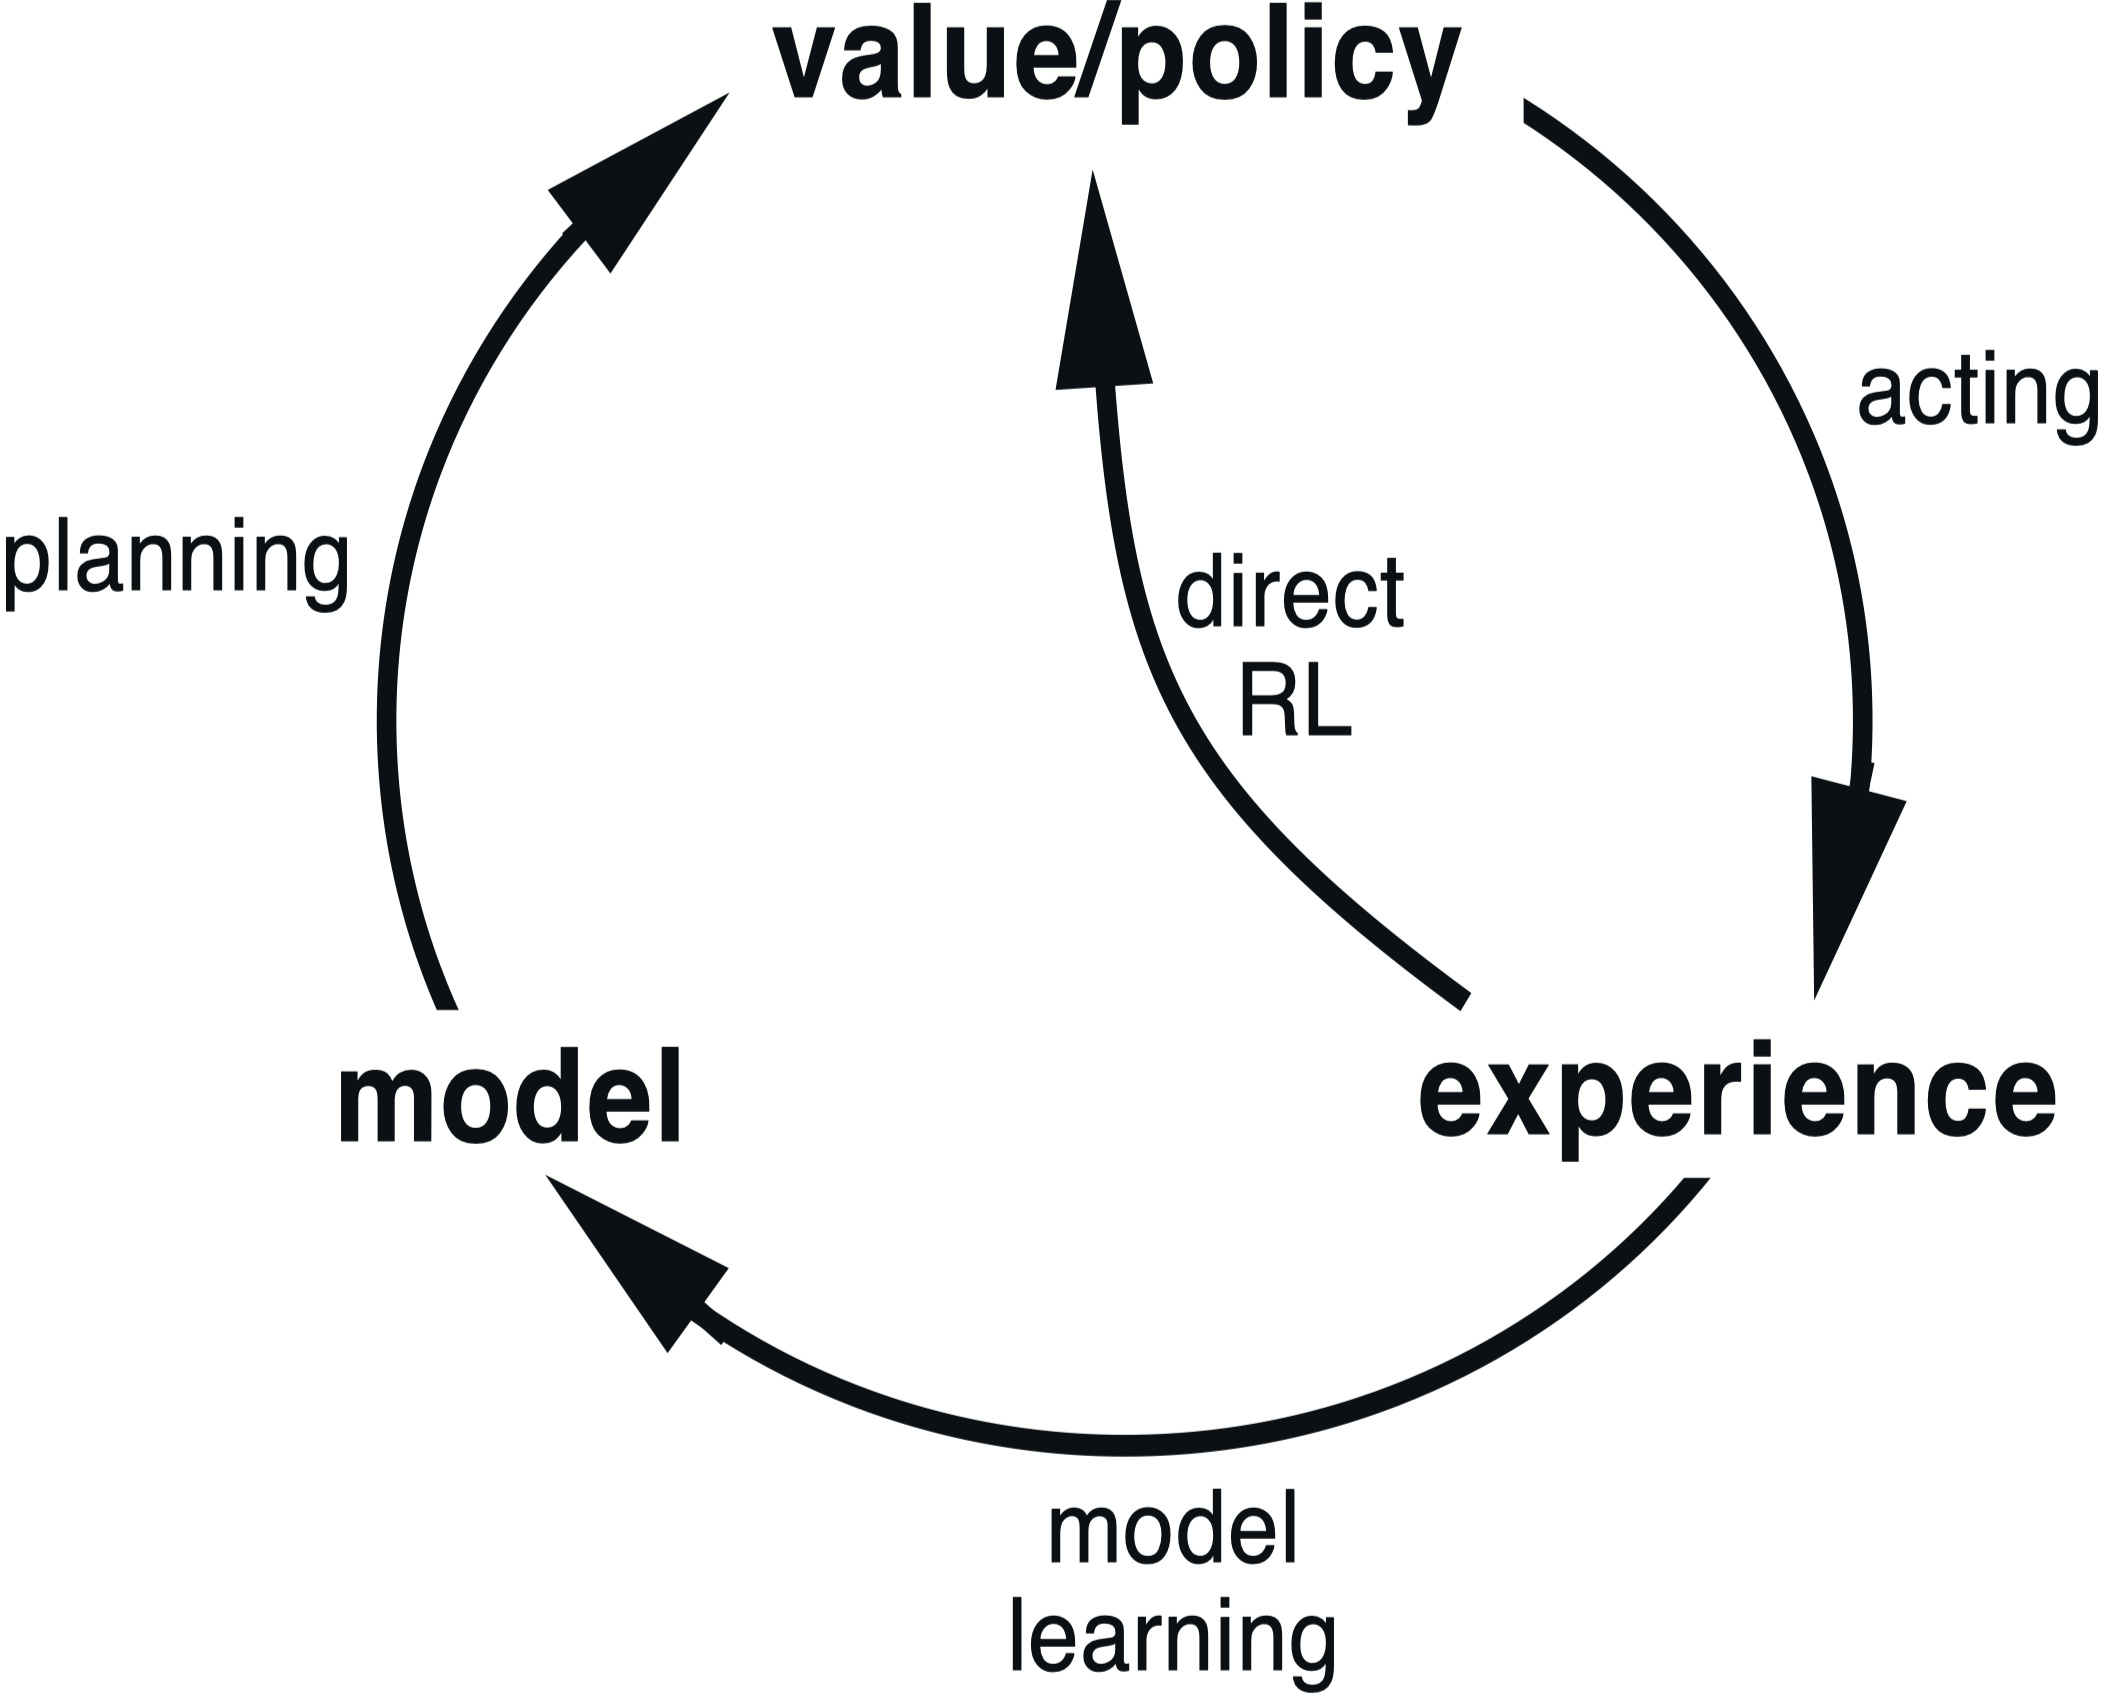
\includegraphics[width=0.66\textwidth]{figures/Dyna.png}
\caption{基于模型的强化学习基本框架。}
\label{fig:dyna-structure}
\end{figure}

\subsection{模型学习的优化}

在学得模型之后,最朴素的用法是,将真实环境数据和模型生成数据 混合,然后执行无模型强化学习方法,这一过程可视作一种数据增广的优化方法。更进阶的模型用法是,使用模型进行上下文信息的辅助计算,从而更高效地加速强化学习算法的收敛速度。

虽然基于模型的强化学习算法有较好的样本效率,但由于模型误差,存在一定的局限性,使用这样有偏差的环境模型去预测,进而会带来更大的误差 \cite{zambaldi2018deep}。

在PILCO方法中 \cite{deisenroth2011pilco},通过学习环境的概率模型,从而实现对复杂环境的不确定性捕捉。具体地,PILCO方法使用了高斯过程回归模型来对环境建模 \cite{quinonero2005unifying},得到环境的概率模型$\mathcal{N}\left(\mu(s_t,a_t), \sigma(s_t,a_t)\right)$,基于这一概率模型,得到期望收益
\begin{equation}
    J^\pi=\mathbb{E}_{s_{t+1}}\left[V\left(s_{t+1}\right)\right]=\int V\left(s_{t+1}\right) \mathcal{N}\left(s_{t+1} \mid \mu_t, \sigma_t\right) \mathrm{d} s_{t+1}
\end{equation}
进而基于梯度$\dfrac{\mathrm{d}J}{\mathrm{d}\theta}$进行策略优化,得到最优参数,使得$\theta^* = {\arg\min}_\theta J^{\pi_\theta}$,最终训练得到最优策略$\pi^*=\pi_{\theta^*}$ 。\cite{peters2006policy}

不确定性环境模型将模型的误差以概率分布的形式展现出来,便能在模型的状态预测环节多次采样得到服从概率分布的预测状态,相比于传统的确定性预测模型,能够让强化学习策略更新环节接收到更多样化的样本输入,从而一定程度上抵消模型偏差带来的影响。但由于高斯过程回归并不适合对复杂的高维度环境进行建模,在后续的PETS方法中,提出使用贝叶斯神经网络(BNN)来对复杂环境进行不确定性建模 \cite{Blundell2015WeightNetworks},从而解决了这一问题。如图\ref{fig:BNN}所示,贝叶斯神经网络的权重不再是固定的权值,而是一个概率分布,神经元间的权值将从这些概率分布中采样得到。

\begin{figure}[tbh]
\centering
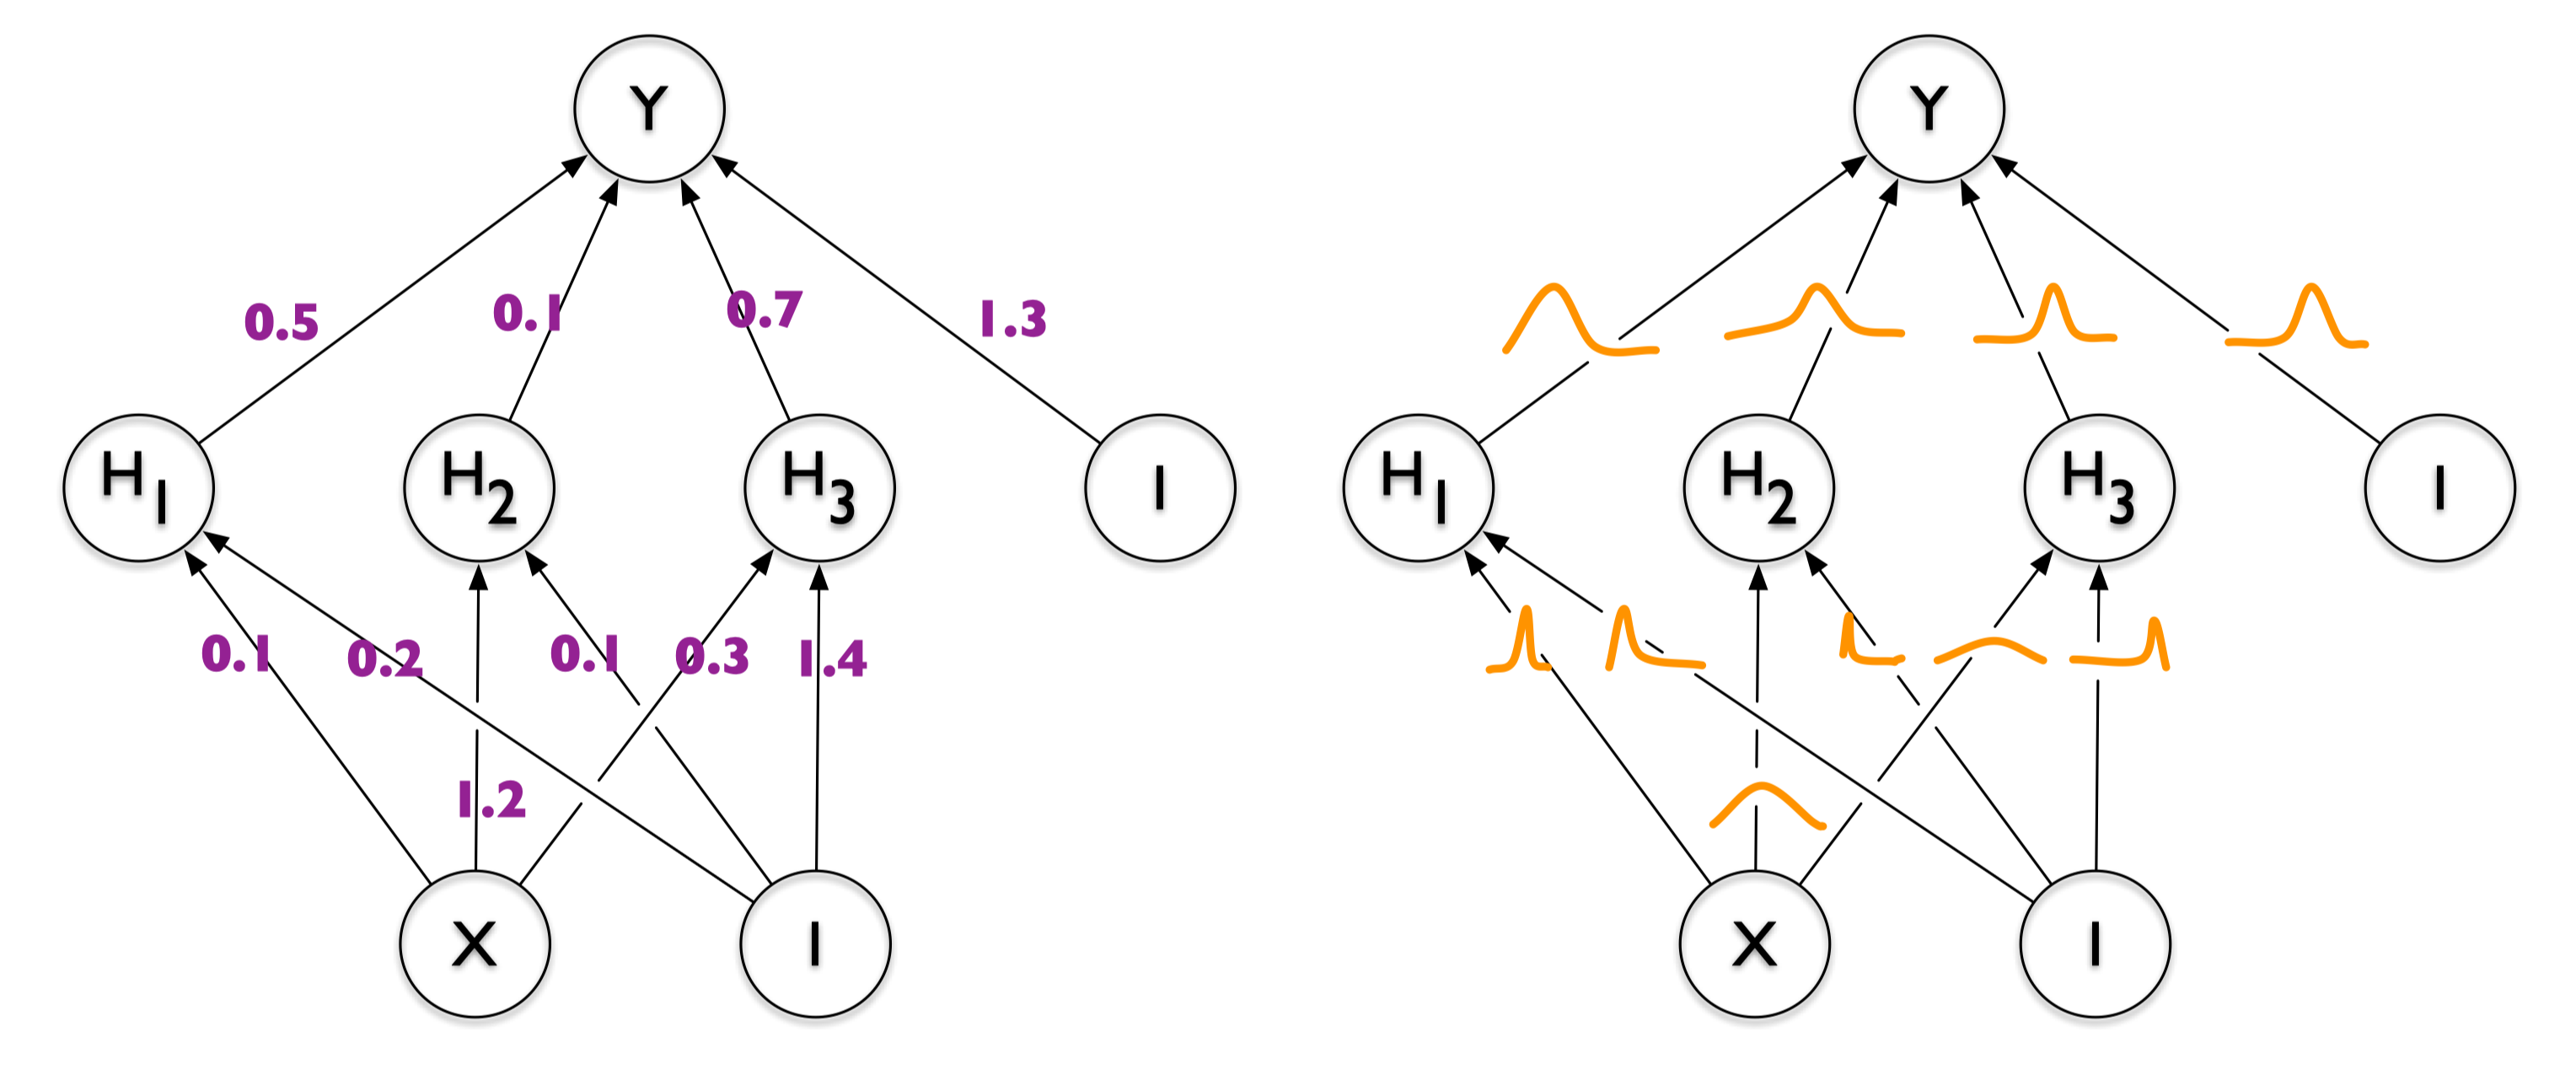
\includegraphics[width=0.9\textwidth]{figures/BNN.png}
\caption{贝叶斯神经网络与普通神经网络的区别。}
\label{fig:BNN}
\end{figure}

\subsection{模型规划的优化}

基于模型的强化学习另一大核心环节便是模型规划 \cite{walsh2010integrating},即使构建出一个准确的环境模型,如果不能合理地利用模型辅助强化学习,对真实样本的利用效率也依然无法得到提升。

在MVE方法中 \cite{feinberg2018model},基于已构建的模型往后展开了$H$步的模拟。由于模型在当前时刻的未来较近步数有着较好的精准度,因此当$H$控制在一个合理范围下时,这$H$步的模拟累积误差相对传统的值函数估计要小很多,将这$H$步模拟替换掉值函数估计,便得到
\begin{equation}
    \hat{V}_{H}\left(s_{0}\right)=\sum_{t=0}^{H-1} \gamma^{t} \hat{r}_{t}+\gamma^{H} \hat{V}\left(\hat{s}_{H}\right)
\end{equation}
MVE将传统无模型强化学习中的值函数学习方法引入模型规划来辅助学习,采用了固定深度的模拟与对剩余部分的估计的结合,实现了模型规划的优化。

在Re-Plan方法中 \cite{williams2017information},每次规划决策得到行动指令,并且基于该指令实际执行行动后,发现真实情况下的转移状态与之前模型规划得到的推理状态之间存在误差,该方法将真实状态进行储存,用作模型预测的修正,从而在下一次规划时,确保模型所预测的有误差状态能被存储记录修正,该方法可以有效地解决模型预测偏差的问题。

而在MBPO方法中 \cite{janner2019trust},证明了当规划长度控制在一个可控长度$k$以内,即

\begin{equation}
k^{*}=\underset{k}{\operatorname{argmin}}\left[\frac{\gamma^{k+1} \epsilon_{\pi}}{(1-\gamma)^{2}}+\frac{\gamma^{k} \epsilon_{\pi}}{(1-\gamma)}+\frac{k}{1-\gamma}\left(\epsilon_{m^{\prime}}\right)\right]>0
\end{equation}

此时,模型的误差始终可以保障在一个误差界限以内,从而在可控的预测误差下,能够最大程度地进行充分的模型规划预测。


\section{本文的主要研究内容}

\section{本文的组织结构}